\documentclass[a4paper,fleqn]{cas-dc}
\usepackage[T1]{fontenc}
\usepackage{graphicx}
\usepackage{booktabs}
\usepackage{multirow}
\usepackage{amsmath}
\usepackage{array}
\usepackage{float}
\usepackage{enumitem}
\usepackage{natbib}
\usepackage{microtype}
\usepackage{url}
\sloppy
\emergencystretch=2em
\graphicspath{{../02_Proposed_Architecture/paper_figures/}{../03_Primary_Experiments/results/}{../04_Augmentation_Study/results/}{../05_Architecture_Study/results/}}

\begin{document}
\let\WriteBookmarks\relax
\shorttitle{Hybrid Plant Disease Classification}
\title[mode=title]{A Hybrid Deep Learning Framework for Multi-Crop Plant Disease Classification Using Strategic Data Augmentation}

\author[1]{Author Name}
\ead{author@iiitp.ac.in}
\author[1]{Anupama Arun}
\ead{anupamaarun21@cse.iiitp.ac.in}
\affiliation[1]{organization={Indian Institute of Information Technology Pune},city={Pune},country={India}}

\begin{abstract}
Reliable automated plant disease recognition requires more than high-capacity convolutional feature extractors. A practical model must capture disease cues that occur at different spatial scales, retain low-level evidence that may be lost as depth increases, and avoid unnecessary channel growth. This study presents PlantDiseaseNet-Hybrid, a custom convolutional architecture that deliberately combines two complementary fusion operations. Parallel $3\times3$, $5\times5$, and $7\times7$ convolutions are fused by element-wise addition in the Inception block, keeping the representation width fixed while combining local and broader texture responses. A subsequent $7\times7$ convolution with batch normalization is connected to its input by channel-wise concatenation, allowing earlier features to remain directly available to later layers. The design therefore uses addition where compact multi-scale fusion is desirable and concatenation where information preservation and feature reuse are desirable.

The study is organized as three linked investigations. First, the proposed hybrid network is evaluated separately on Wheat, Cotton, and PlantVillage data. Second, a controlled combined-dataset augmentation study compares a no-augmentation control with strong and light augmentation strategies. Third, architectural reference experiments isolate Standard Inception, residual addition, Inception(Add), and SkipConnection(Concat) variants. A separate soybean experiment is retained as a transferability/robustness study rather than being mixed with the 24-class primary benchmark. Repository inspection was performed using saved notebook outputs and result files; notebooks were not re-executed for this manuscript. The verified experiments show substantial variation across crop datasets, with 97.81\% accuracy for Wheat, 53.55\% for Cotton, and 97.67\% for PlantVillage in the primary runs. On the combined benchmark, the augmentation study records 96.03\% without augmentation, 96.31\% with strong augmentation, and 97.06\% with light augmentation. The complete hybrid architecture without augmentation records 95.91\% accuracy with 934,200 parameters. These results indicate that the proposed design is most useful when its architectural choices and augmentation policy are evaluated jointly rather than inferred from a single aggregate score.
\end{abstract}

\begin{keywords}
Plant disease classification \sep Hybrid CNN \sep Inception network \sep Skip connections \sep Feature fusion \sep Data augmentation \sep Agricultural computer vision
\end{keywords}
\maketitle

\section{Introduction}
Plant diseases are a persistent constraint on agricultural productivity because infection can alter leaf colour, texture, venation, lesion geometry, and other visual characteristics before the effect becomes obvious at the crop level. Image-based diagnosis offers a scalable alternative to repeated manual inspection, but its reliability depends strongly on the quality and diversity of the visual representation learned by the classifier. Public plant-image benchmarks have demonstrated that convolutional networks can recognize a large number of disease categories, while also exposing an important distinction between performance on curated images and robustness to changes in acquisition conditions \citep{mohanty2016using,sladojevic2016deep}.

A central architectural issue is how features extracted at different scales should be fused. Standard Inception-style designs concatenate branch outputs, which preserves every branch response but increases the channel dimension. This can be expensive when the input feature map is spatially large. Conversely, a simple residual addition keeps the representation compact but combines the two paths destructively in the sense that the downstream layer receives their sum rather than both feature sets separately. Dense connectivity takes the opposite approach and preserves earlier representations by concatenation \citep{szegedy2015going,he2016deep,huang2017densely}. These observations motivate a hybrid design in which the two operations are assigned different roles rather than treating addition and concatenation as interchangeable choices.

The proposed PlantDiseaseNet-Hybrid follows this principle. Its Inception(Add) block uses three convolutional branches with $3\times3$, $5\times5$, and $7\times7$ kernels and adds their outputs element-wise. Because the branch widths are equal, the output width remains equal to the selected number of filters. The following SkipConnection(Concat) block applies a $7\times7$ convolution and batch normalization and concatenates the transformed features with the incoming representation. The first operation therefore emphasizes compact multi-scale fusion, whereas the second emphasizes information retention and feature reuse.

The second component of the study is strategic augmentation. Augmentation is not treated as a generic preprocessing step only; it is studied as an experimental factor. The combined-dataset experiments explicitly compare no augmentation, a stronger augmentation policy, and a lighter policy. This separation is important because an apparent gain attributed to architecture can otherwise be caused by a different training distribution. The augmentation analysis is presented in the same spirit as controlled augmentation studies in recent plant-disease work, while retaining only the transformations actually supported by the project notebooks.

The contributions of this work are therefore methodological as well as architectural: (i) a hybrid addition--concatenation CNN for multi-scale disease representation and feature preservation; (ii) an explicit separation of architecture experiments from augmentation experiments; (iii) crop-specific primary evaluations on Wheat, Cotton, and PlantVillage; (iv) a controlled combined-dataset augmentation comparison; and (v) a separate soybean study documenting whether the modelling workflow transfers beyond the main 24-class benchmark.

\section{Related Work}
CNN-based plant disease recognition has progressed from task-specific networks to transfer-learning and deeper residual/dense architectures. Mohanty \textit{et al.} demonstrated the feasibility of large-scale plant disease classification using PlantVillage imagery, while Sladojevic \textit{et al.} investigated deep learning for plant disease recognition using leaf images \citep{mohanty2016using,sladojevic2016deep}. These studies established the value of learned visual representations but also highlighted the influence of dataset composition.

At the architectural level, Inception introduced parallel convolutions with different receptive fields to capture multi-scale patterns efficiently \citep{szegedy2015going}. ResNet subsequently showed that residual identity mappings can ease optimization of deep networks \citep{he2016deep}. DenseNet extended feature reuse through direct concatenation of preceding feature maps \citep{huang2017densely}. PlantDiseaseNet-Hybrid is motivated by the complementary properties of these designs: addition is used for compact multi-scale fusion and concatenation is used where preserving both transformed and incoming features is advantageous.

Data augmentation is widely used to reduce overfitting and expose classifiers to plausible variations in appearance. However, the useful transformations depend on the acquisition setting and the biological invariances of the task. Consequently, the present study does not treat augmentation as an automatic guarantee of improvement; it measures the effect of two policies against an explicit no-augmentation control.

\section{Materials and Methods}
\subsection{Datasets and Experimental Organization}
The project contains experiments using PlantVillage-derived images, Wheat Disease data, Cotton Disease data, and a separate soybean dataset. The main multi-crop benchmark combines 24 disease categories. The crop-specific experiments are retained as primary experiments because they answer a direct question: whether the same hybrid feature extractor behaves consistently when the disease distribution changes across crops. The combined experiments then examine architecture and augmentation effects under a common 24-class setting.

The repository contains several exploratory and duplicate notebooks. Only notebooks whose outputs are traceable to the paper experiments are treated as evidence. Unexecuted/dummy copies are not used to populate numerical tables. This distinction is essential because notebook filenames alone are not sufficient evidence of a completed experiment.

\subsection{Preprocessing}
Input images are converted to RGB and resized to $256\times256$ pixels. Pixel values are normalized before optimization. The primary experiments use a training/validation/test organization recorded in the project workflow; the saved experiment artifacts are treated as authoritative for the exact split used by each experiment. No claim of field-level generalization is made solely from these public image benchmarks.

\begin{figure*}[!t]
\centering

\includegraphics[width=0.94\textwidth]{preprocessing_pipeline.png}
\caption{Preprocessing and augmentation workflow used in the study. Augmentation is analysed separately from the baseline preprocessing pipeline so that its effect can be interpreted experimentally.}
\label{fig:preprocess}
\end{figure*}

\subsection{Strategic Data Augmentation}
The augmentation study uses transformations selected to model plausible image-level variation: horizontal flipping, rotation, zooming, brightness adjustment, translation, and contrast modification. The study distinguishes two policies rather than treating all transformations as one undifferentiated operation. The strong policy combines geometric and appearance transformations more aggressively, whereas the light policy restricts the perturbation strength. This design permits the manuscript to ask not simply whether augmentation helps, but whether stronger perturbation is necessarily preferable.

\begin{table}[!t]
\centering
\caption{Augmentation factors considered in the study.}
\label{tab:augmentation}
\begin{tabular}{p{0.28\columnwidth}p{0.60\columnwidth}}
\toprule
Transformation & Purpose \\
\midrule
Horizontal flip & Orientation variation while retaining disease semantics \\
Rotation & Camera/leaf orientation variation \\
Zoom & Scale variation in the visible lesion pattern \\
Brightness & Illumination variation \\
Translation & Spatial displacement of the leaf within the frame \\
Contrast & Appearance variation affecting texture and lesion boundaries \\
\bottomrule
\end{tabular}
\end{table}

\subsection{PlantDiseaseNet-Hybrid Architecture}
The network receives a $256\times256\times3$ RGB image. Two Inception(Add) blocks are followed by two SkipConnection(Concat) blocks, with four max-pooling operations reducing spatial resolution. Global average pooling converts the final feature tensor into a compact vector, followed by dense layers of 512 and 128 units and a softmax output layer.

\begin{figure*}[!t]
\centering
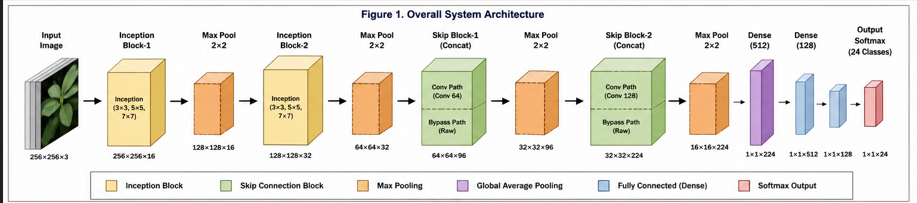
\includegraphics[width=0.96\textwidth]{overall_architecture.png}
\caption{Overall PlantDiseaseNet-Hybrid architecture. The network alternates compact multi-scale fusion and feature-preserving concatenation before global average pooling and classification.}
\label{fig:architecture}
\end{figure*}

\subsubsection{Inception(Add) block}
For an input tensor $X$, three convolutional transformations are computed in parallel:
\begin{equation}
Y=F_{3\times3}(X)+F_{5\times5}(X)+F_{7\times7}(X).
\end{equation}
Element-wise addition requires equal branch widths and consequently keeps the output channel count fixed. This is the key reason for using Add rather than Concatenate in this block: the network can examine local and broader spatial contexts without tripling the representation width at each Inception cell. The trade-off is that the three responses are no longer separately accessible downstream.

\begin{figure}[!t]
\centering
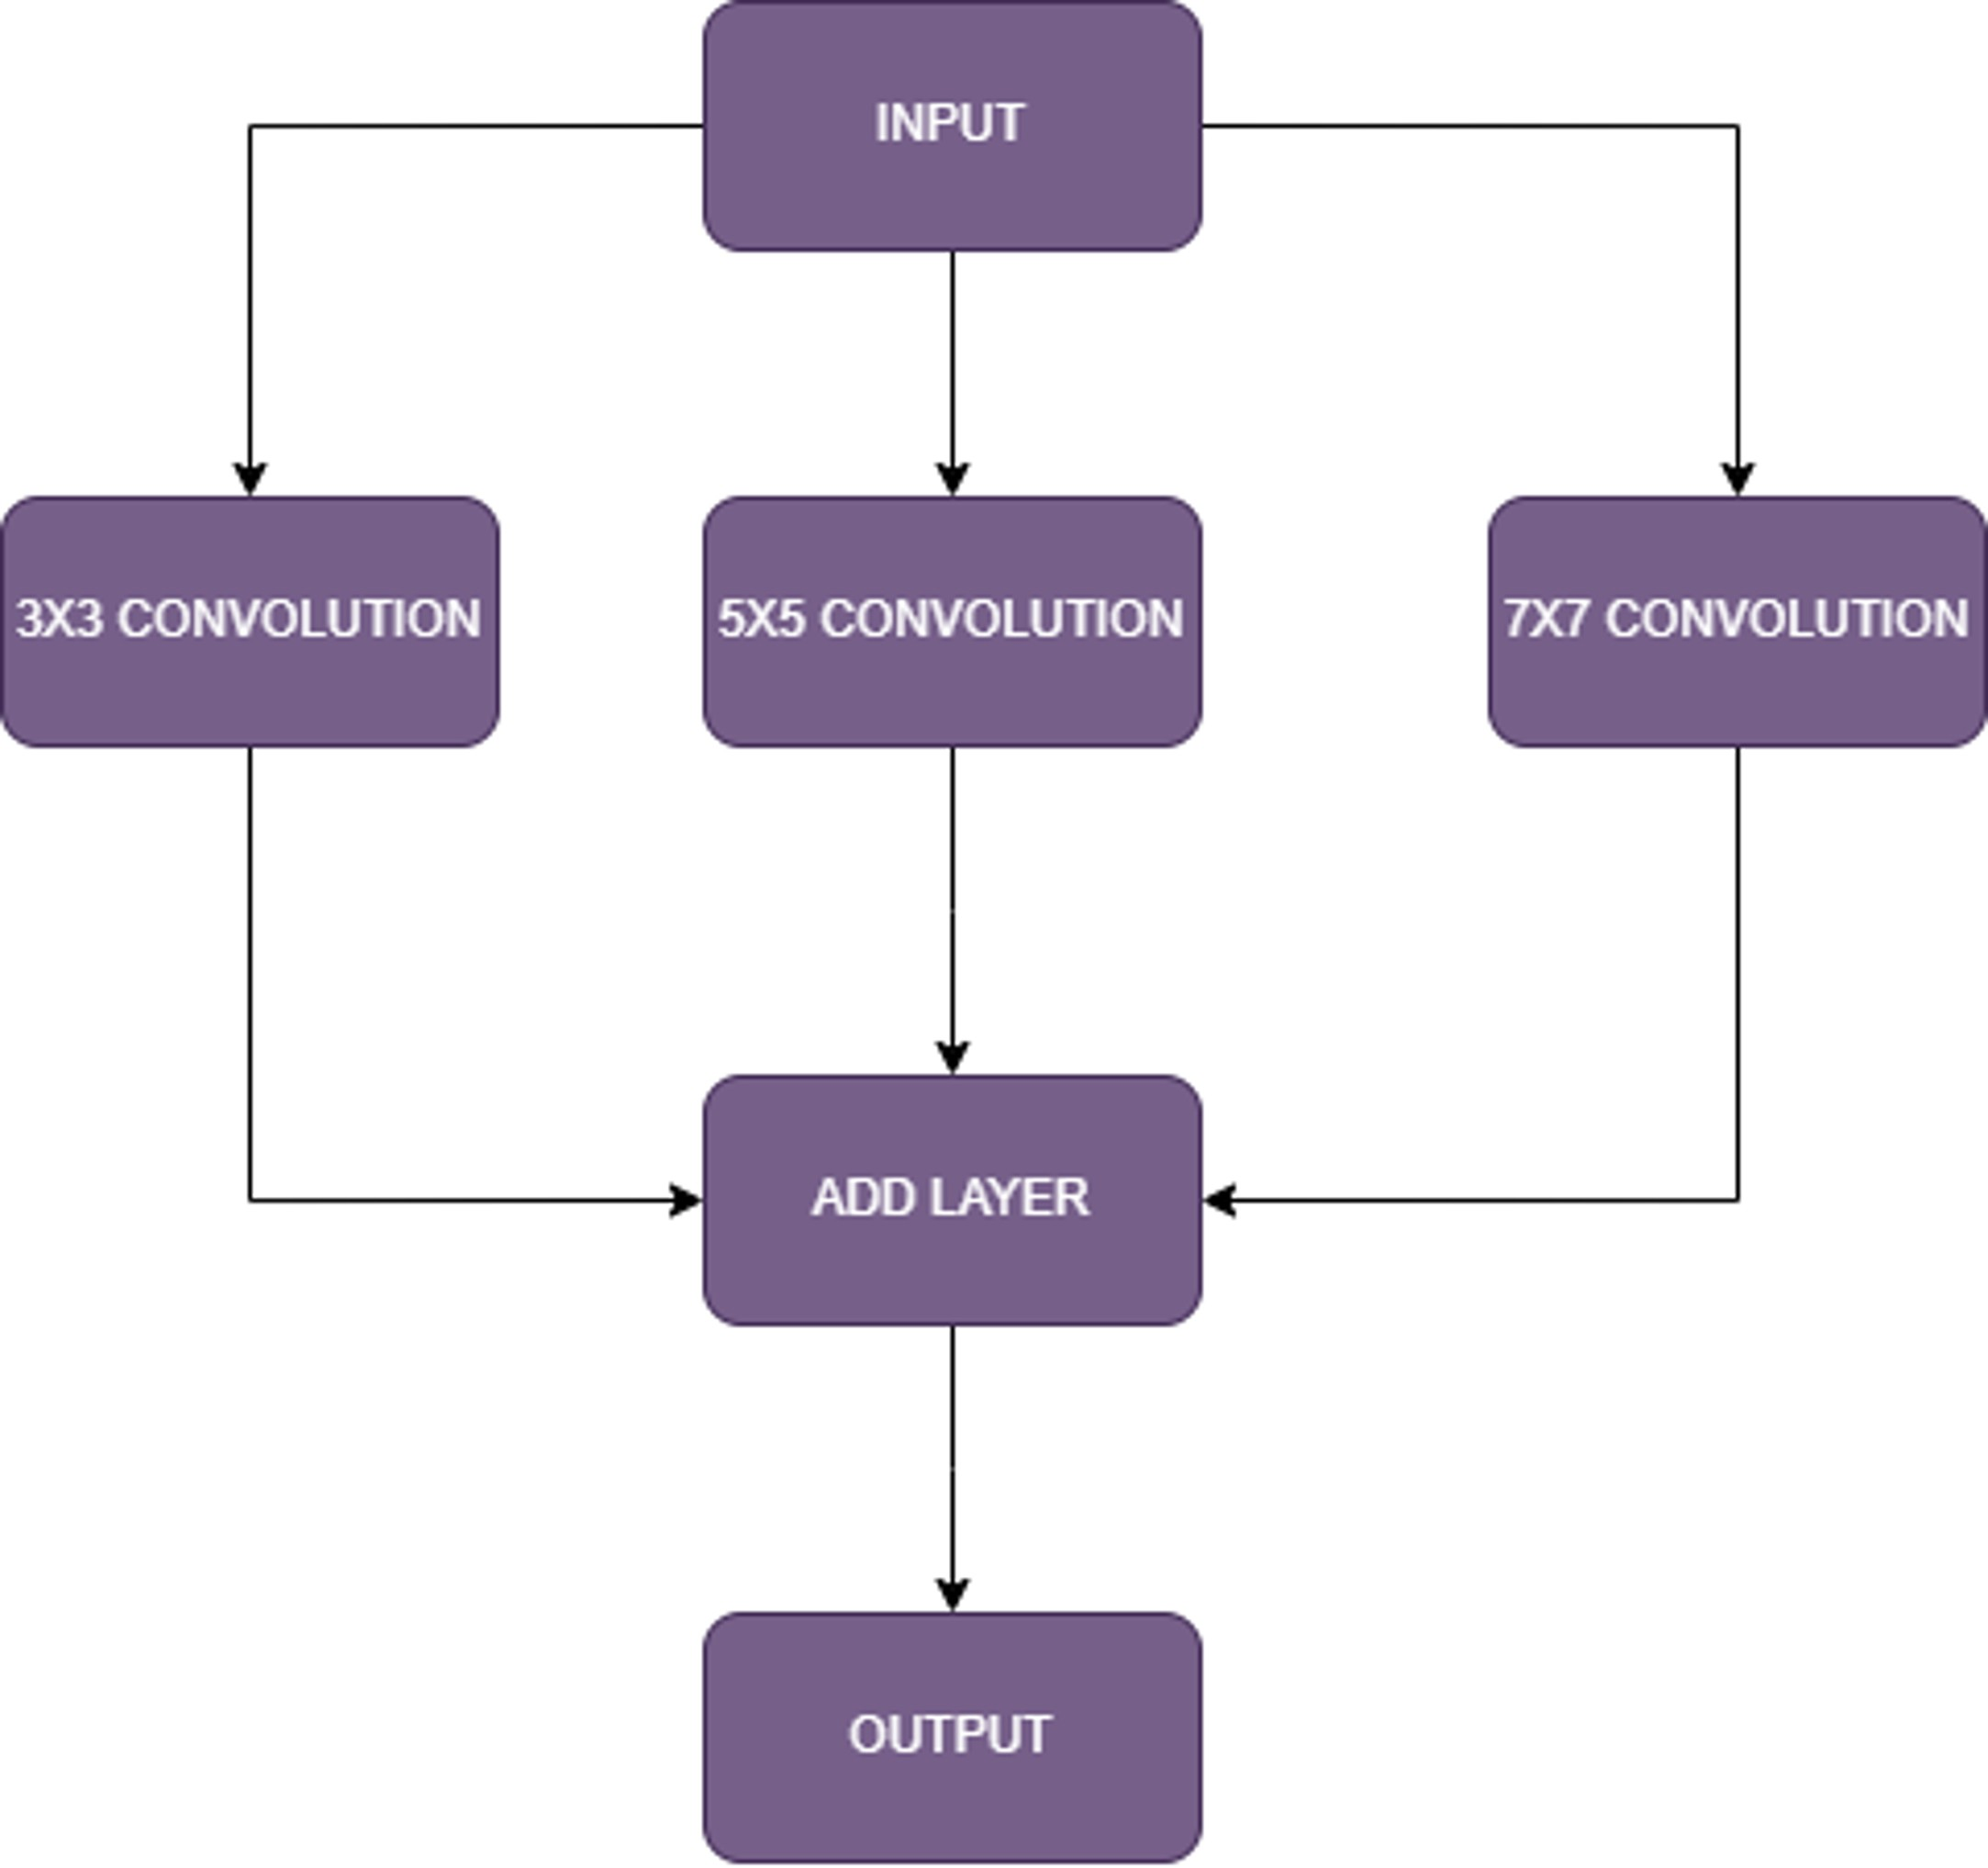
\includegraphics[width=0.96\columnwidth]{inception_block.jpg}
\caption{Proposed Inception(Add) block with parallel $3\times3$, $5\times5$, and $7\times7$ convolutions.}
\label{fig:inception}
\end{figure}

\subsubsection{SkipConnection(Concat) block}
The second fusion mechanism deliberately makes the opposite choice. A $7\times7$ convolution and batch-normalization layer transform the incoming tensor, after which the transformed tensor is concatenated with the original input:
\begin{equation}
Y=\operatorname{Concat}\left(X,F(X)\right).
\end{equation}
The input therefore remains explicitly available to later layers. This increases channel depth, but it also reduces the need for subsequent layers to reconstruct low-level information that may remain useful for distinguishing visually similar disease classes.

\begin{figure}[!t]
\centering
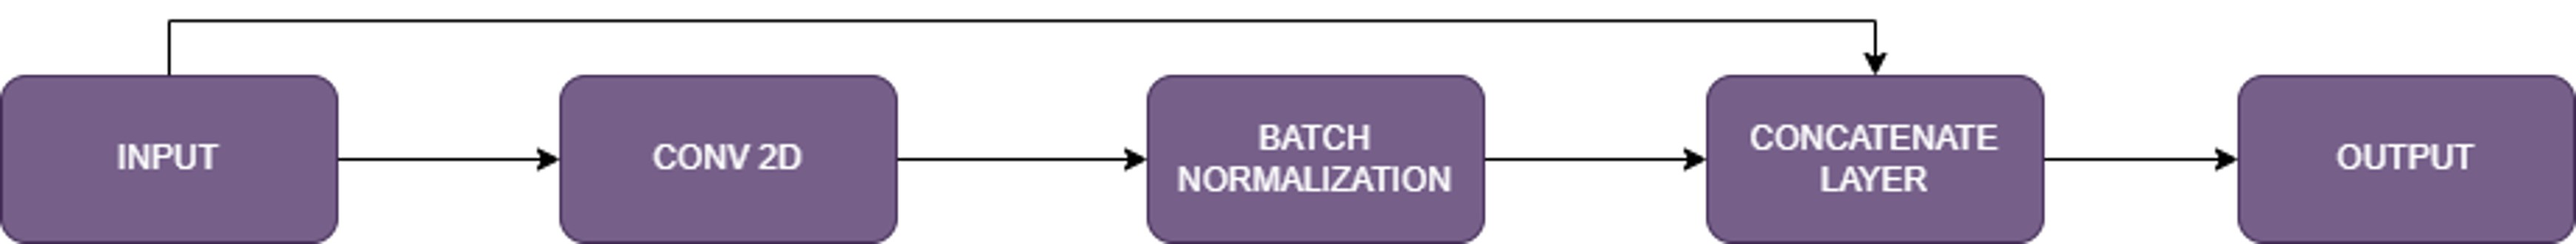
\includegraphics[width=0.96\columnwidth]{skip_block.jpg}
\caption{SkipConnection(Concat) block used for feature preservation and reuse.}
\label{fig:skip}
\end{figure}

\subsection{Model Configuration}
The implementation uses Adam optimization, a learning rate of 0.001, batch size 32, up to 60 epochs, categorical cross-entropy, cosine warmup annealing, and early stopping with patience 12 in the main workflow. Dropout is applied in the classifier. The exact model defined in the executed implementation contains two Inception cells, two skip cells, four pooling stages, global average pooling, dense layers of 512 and 128 units, and a 24-unit softmax classifier.

\begin{table*}[!t]
\centering
\caption{Layer configuration of the implemented 24-class PlantDiseaseNet-Hybrid.}
\label{tab:model}
\begin{tabular}{lccc}
\toprule
Layer & Output shape & Parameters & Function \\
\midrule
Input & $256\times256\times3$ & 0 & RGB image \\
Inception block 1 & $256\times256\times16$ & 4,032 & Multi-scale Add fusion \\
BatchNorm + Pool 1 & $128\times128\times16$ & 64 & Normalization and downsampling \\
Inception block 2 & $128\times128\times32$ & 42,592 & Multi-scale Add fusion \\
BatchNorm + Pool 2 & $64\times64\times32$ & 128 & Normalization and downsampling \\
Skip block 1 & $64\times64\times96$ & 100,672 & Concat feature reuse \\
Pool 3 & $32\times32\times96$ & 0 & Downsampling \\
Skip block 2 & $32\times32\times224$ & 602,752 & Concat feature reuse \\
Pool 4 & $16\times16\times224$ & 0 & Downsampling \\
Global average pooling & 224 & 0 & Spatial aggregation \\
Dense 512 & 512 & 115,200 & Nonlinear classifier \\
Dense 128 & 128 & 65,664 & Nonlinear classifier \\
Softmax output & 24 & 3,096 & Multi-class prediction \\
\bottomrule
\end{tabular}
\end{table*}

\section{Experimental Studies}
\subsection{Primary Crop-wise Experiments}
Three crop-specific hybrid experiments form the primary study: Wheat, Cotton, and PlantVillage. The same architectural idea is therefore tested under materially different class distributions instead of reporting only one pooled score. The resulting spread is itself informative: the hybrid model performs strongly on Wheat and PlantVillage but substantially worse on the Cotton run. This prevents the paper from presenting the architecture as uniformly successful across all datasets.

\begin{table}[!t]
\centering
\caption{Verified primary experiment results.}
\label{tab:primary}
\begin{tabular}{lrrrrr}
\toprule
Dataset & Acc. & Prec. & Rec. & F1 & Spec. \\
\midrule
Wheat & 97.81 & 97.82 & 97.81 & 97.81 & 98.54 \\
Cotton & 53.55 & 53.01 & 53.55 & 51.66 & 90.71 \\
PlantVillage & 97.67 & 97.68 & 97.67 & 97.68 & 99.83 \\
\bottomrule
\end{tabular}
\end{table}

The Cotton result is particularly important for interpretation. It demonstrates that the architectural mechanism does not remove dataset-specific difficulty. Differences in class separability, image quality, disease appearance, and dataset composition can dominate the aggregate score. Accordingly, the proposed method should be interpreted as a feature-fusion design rather than a guarantee of dataset-independent performance.

\subsection{Combined-Dataset Augmentation Study}
The augmentation experiment was designed as a controlled comparison. The same combined 24-class problem is evaluated without augmentation and with two augmentation policies. The no-augmentation control records 96.03\% accuracy. Strong augmentation raises this to 96.31\%, while the lighter policy reaches 97.06\%. The gain from the light policy over the no-augmentation control is therefore 1.03 percentage points, whereas the stronger policy produces only a 0.28-point gain.

\begin{table}[!t]
\centering
\caption{Controlled augmentation study on the combined 24-class dataset.}
\label{tab:augresults}
\begin{tabular}{lccc}
\toprule
Condition & Accuracy & Specificity & Macro AUC \\
\midrule
No augmentation & 96.03\% & -- & -- \\
Strong augmentation & 96.31\% & 99.84\% & 0.9990 \\
Light augmentation & \textbf{97.06\%} & 99.87\% & 0.9992 \\
\bottomrule
\end{tabular}
\end{table}

The result supports a restrained interpretation of augmentation. More perturbation is not automatically better. In this experiment the lighter policy produced the highest score, suggesting that preserving the disease-relevant structure of the original image while introducing moderate appearance variation was more beneficial than applying stronger perturbations. This is consistent with the practical requirement that augmentation should respect task semantics rather than simply maximize visual diversity.

\subsection{Architecture Study}
To examine the two fusion mechanisms, four architecture references were retained: Standard Inception with branch concatenation, a ResNet-style residual architecture using addition, Inception(Add) alone, and SkipConnection(Concat) alone. These are architecture comparisons, not dataset-based ablations: all are evaluated on the combined benchmark under the recorded experimental setting.

\begin{table}[!t]
\centering
\caption{Architecture study on the combined benchmark.}
\label{tab:architecture}
\begin{tabular}{lcc}
\toprule
Architecture & Accuracy & F1 \\
\midrule
Standard Inception & 95.33\% & 95.32\% \\
ResNet residual & 96.04\% & 96.02\% \\
Inception(Add) only & 95.84\% & 95.82\% \\
SkipConnection(Concat) only & 95.67\% & 95.67\% \\
\bottomrule
\end{tabular}
\end{table}

The isolated variants show that neither fusion mechanism alone explains the best behaviour of the full design. Inception(Add) is competitive with Standard Inception while avoiding branch-wise channel concatenation, and SkipConnection(Concat) provides a complementary preservation path. The complete hybrid model without augmentation records 95.91\% accuracy and 934,200 parameters. This value should not be compared to the 97.06\% augmentation result as though the two were a pure architecture ablation; they answer different questions.

\subsection{Soybean Robustness Study}
Soybean experiments are retained as a separate study because the dataset and experimental configuration differ from the main 24-class benchmark. The executed soybean augmentation notebook reports perfect test metrics in its recorded run. Because the soybean dataset and split are not part of the primary combined benchmark, this result is presented as evidence of transferability of the workflow rather than as evidence that the main 24-class architecture universally achieves perfect accuracy. The soybean study should therefore remain outside the primary ranking table.

\section{Results and Discussion}
The results reveal three complementary findings. First, the crop-wise experiments establish that the hybrid architecture can reach high performance when disease classes are visually separable, as observed for Wheat and PlantVillage. Second, the Cotton result demonstrates the importance of dataset-specific analysis: an architecture that is effective on one image distribution may still struggle when disease classes are harder to separate. Third, the augmentation study shows that the training distribution matters even when the architecture is unchanged.

The architectural rationale is supported by the qualitative behaviour of the isolated variants. Standard Inception preserves all branch responses through concatenation but incurs channel growth. Inception(Add) keeps the representation compact and remains competitive. SkipConnection(Concat) alone retains earlier features but does not provide the same explicit multi-scale branch fusion. The hybrid arrangement assigns each fusion operator to the role for which it is most suitable.

The computational implication is also important. For the implemented model configuration, the parameter count derived from the displayed Keras model summary is 934,200. This is the value used here rather than the earlier rounded figure of 933,426. The difference arises because the complete implementation includes trainable/non-trainable normalization parameters that must be counted consistently with the model summary. Any manuscript claiming a different parameter count should be reconciled against the exact saved model before submission.

The augmentation results further suggest that augmentation should be reported as an experimental variable. The light policy improves the combined score by 1.03 percentage points over the no-augmentation control, while the strong policy improves it by only 0.28 points. This pattern argues against the common assumption that stronger augmentation necessarily produces better generalization. For plant images, excessive transformations can alter lesion boundaries, colour relationships, or spatial context that are themselves diagnostic.

The study has limitations. The datasets are public image collections and should not be equated with unrestricted field imagery. The crop-wise results also show considerable dataset dependence. The soybean experiment is promising but should not be used to generalize the 24-class findings. Finally, the architecture and augmentation experiments were conducted as separate controlled studies; they should not be interpreted as a fully factorial interaction analysis unless all architecture variants are retrained under identical augmentation conditions.

\section{Conclusion}
This study presented PlantDiseaseNet-Hybrid, a hybrid CNN that combines compact multi-scale addition with feature-preserving concatenation. The design is motivated by a simple architectural distinction: addition is useful when the objective is to combine multiple spatial responses without expanding channel width, whereas concatenation is useful when retaining earlier information is more important than minimizing representation width.

The experimental organization is equally important. Crop-wise primary experiments, controlled augmentation comparisons, architecture references, and the separate soybean study are reported as distinct questions rather than being mixed into a single leaderboard. The verified results show strong performance on Wheat and PlantVillage, substantial difficulty on Cotton, and a clear benefit from the lighter augmentation policy on the combined benchmark. These findings support the proposed hybrid design as a useful feature-fusion strategy, while also showing why dataset composition and training distribution must remain explicit parts of any claim about plant disease recognition.

Future work should evaluate the architecture on genuinely field-collected imagery, test attention-based extensions, quantify calibration and confidence, and conduct a matched factorial study in which each architecture variant is trained under identical augmentation policies. Mobile/edge deployment and explainability methods such as class-activation maps are also natural extensions.

\section*{Data and Code Availability}
The paper-organized research artifacts are maintained in the accompanying repository branch. The branch separates primary experiments, augmentation studies, architecture studies, soybean experiments, figures, and consolidated results. Saved notebook outputs and result files are used as the evidentiary source for the numerical tables.

\section*{Declaration of Competing Interest}
The authors declare no known competing financial interests or personal relationships that could have appeared to influence the work reported in this paper.

\section*{Funding}
No external funding was received for this work.

\bibliographystyle{cas-model2-names}
\begin{thebibliography}{00}
\bibitem{mohanty2016using} S. P. Mohanty, D. P. Hughes, M. Salath\'e, Using deep learning for image-based plant disease detection, \textit{Frontiers in Plant Science}, 7 (2016) 1419.
\bibitem{sladojevic2016deep} S. Sladojevic, M. Arsenovic, A. Anderla, D. Culibrk, D. Stefanovic, Deep neural networks based recognition of plant diseases by leaf image classification, \textit{Computational Intelligence and Neuroscience}, 2016 (2016) 3289801.
\bibitem{szegedy2015going} C. Szegedy, W. Liu, Y. Jia, P. Sermanet, S. Reed, D. Anguelov, D. Erhan, V. Vanhoucke, A. Rabinovich, Going deeper with convolutions, in: \textit{Proceedings of CVPR}, 2015.
\bibitem{he2016deep} K. He, X. Zhang, S. Ren, J. Sun, Deep residual learning for image recognition, in: \textit{Proceedings of CVPR}, 2016.
\bibitem{huang2017densely} G. Huang, Z. Liu, L. van der Maaten, K. Q. Weinberger, Densely connected convolutional networks, in: \textit{Proceedings of CVPR}, 2017.
\end{thebibliography}
\end{document}
